%!TEX root = ../main.tex
% !TeX encoding = UTF-8
\section{Princípios do Particionamento de Sistemas Gerais} \label{chap:design}
    
    A seguir serão descritos tópicos utilizados para o entendimento do particionamento, seguindo conceitos estabelecidos por vários trabalhos como \cite{Arato2003, Arato2005, Mann2007, BenHajHassine2017, Sass2010}.
    Esses tópicos são necessários para o entendimento básico dos arcabouços metodológicos de \codesign\ e o seu particionamento para sistemas, em especial para \wearables, além de definições formais sobre.
    
    %Os tópicos a seguir são a Definição de \Design\ de Referência de \Software\ (Seção~\ref{sec:GCF}) bem como o Ganho de Performance (Seção~\ref{sec:ganho_performance}) em tais sistemas, o Particionamento \HS\ para Sistemas \Wearables\  (Seção~\ref{sec:desenvolvimento}) e a Proposta de Procedimento Analítico (Seção~\ref{sec:proposta}).
    
    %\subsection{Fundamentação Matemática} \label{sec:GCF}
    
    É possível descrever sistemas livre de especificações formais por meio de descrições de protótipos simples, conhecidos como \Design\ de Referência de \Software\ (DRS)\cite{Sass2010}.
    %Com ele, é possível ter uma generalização de uma especificação sistêmica, eliminando quaisquer tipo de incertezas sobre o comportamento do sistema ao realizar uma análise sobre, sendo este podendo ser representado por diversas formas.
    % além de outras como o fato de que sua especificação pode ser analisada por ferramentas computacionais, e gerando modelos aut.
    %
    %Assumindo que o \design\ de referência de \textit{software} já exista,
    %Primeiramente, será demonstrado matematicamente como computação está em \design\ referencial de \sof%htware\ para que depois, isso possa nos auxiliar na decisão do que deverá ser implementado em nível de \hs.
    Dessa forma, o algoritmo a ser analisado também pode ser representado como grafo de rotinas, chamado de Grafo de Controle de Fluxo (GCF) \cite{Mann2007}.
    Ele é definido por $C = (B, F) \label{eq:subrotina}$
    %\begin{equation}
    %   C = (B, F) \label{eq:subrotina}
    %\end{equation}
    onde $B$ são vértices que representam as tarefas %\footnote{De modo geral é um trecho de código sequencial maximal, onde só existe um ponto de entrada e um ponto de saída.}
    %http://www.dcc.ufrj.br/~gabriel/microarq/Escalonamento.pdf
    e $ F $ são arestas que indicam todas as possibilidades de caminhos entre elas.
    
    \begin{comment} %figura
    Utilizando o exemplo da Figura \ref{fig:blocos_basicos}, o primeiro grupo \A\ é um bloco não básico porque não é maximal, ou seja, a primeira instrução \texttt{store word with update} deveria estar incluída ao grupo para conter o número máximo de instruções possuindo apenas um ponto de entrada e saída.
    Grupo \B\ é um bloco básico e o grupo \C\ não se define como bloco básico pois existe duas entradas para o bloco, sendo elas na instrução \texttt{store word} e também pelo \texttt{branching} direcionado para \texttt{L2}.
    
    Dessa forma, fazendo uma relação entre o processo de gerar um Grafo de Controle de Fluxo a partir de um código em alto nível, a Figura~\ref{fig:f3-6} exibe um pequeno código demonstrativo na qual o processo ocorrerá.
    A partir do código em alto nível (Figura~\ref{fig:f3-6} \textit{a)}) é identificado os blocos básicos de acordo com o compilador\footnote{Deve-se atentar que, só é possível identificar blocos básicos em um arquivo em linguagem de programação \textit{C} desde que se saiba qual compilador foi utilizado para emitir o código \assembly.} utilizado.
    Neste exemplo, utilizou-se de um compilador para \texttt{PowerPC}\footnote{Arquitetura que utiliza RISC como arquitetura do conjunto de instruções.} onde os blocos básicos são identificados pela Figura~\ref{fig:f3-6} \textit{b)}.
    Por fim o GCF resultante deste processo, representado pela Figura~\ref{fig:f3-6} \textit{c)}.
    
    \begin{figure}[!ht] \centering
    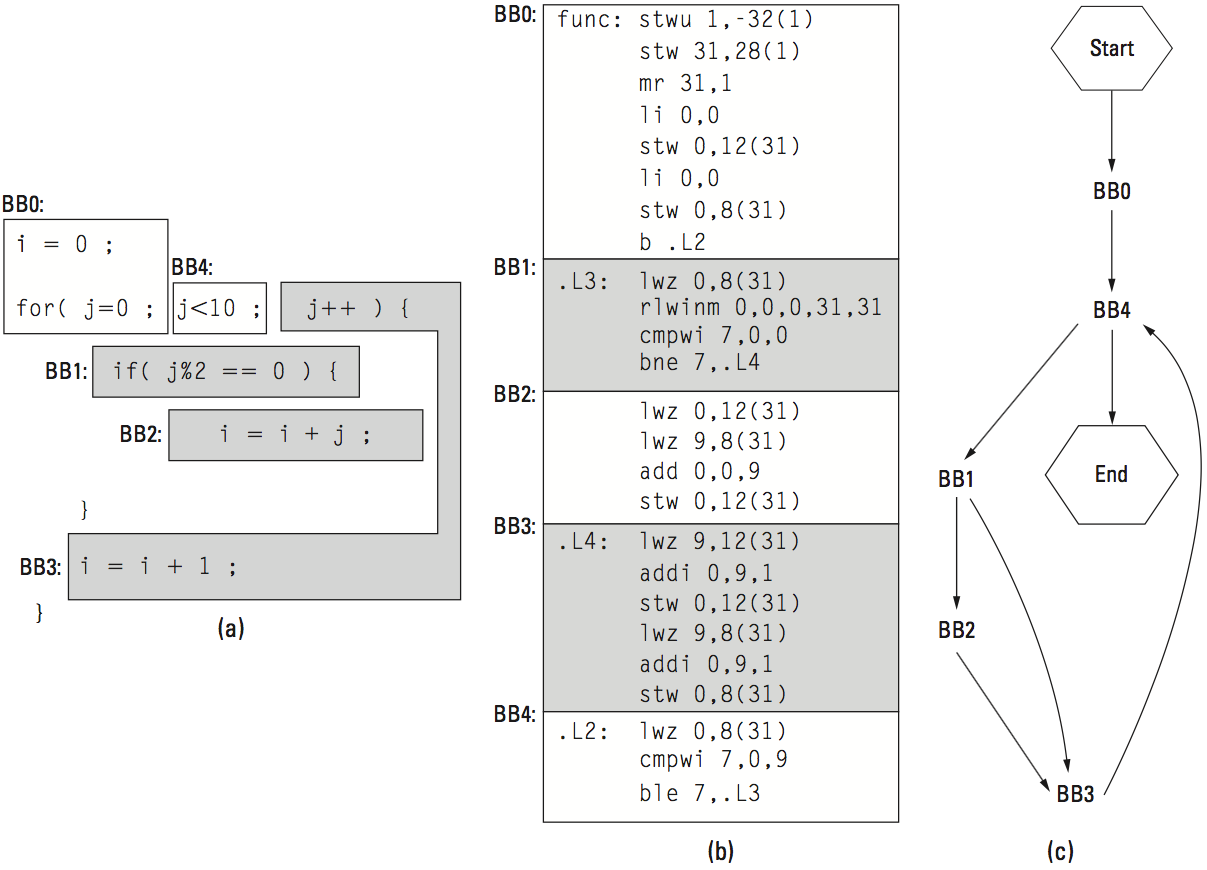
\includegraphics[width=0.35\textwidth]{img/f3-6.png}
    \caption{Identificação de blocos básicos e a representação por meio de um grafo não atrelado à uma especificação \hs.}
    \label{fig:f3-6}
    \end{figure}
    \end{comment}
    
    A decomposição de um DRS pode gerar dois componentes: uma porção a ser realizada em \hardware\ e outra executada em \software.
    Essa decisão de divisão é chamada de Problema de Particionamento.
    %Segundo \cite{Sass2010}, para sistemas em FPGA, o particionamento é um sub-problema de um problema mais geral no âmbito de \codesign, onde refere-se ao \design\ cooperativo entre engenheiros de \hs\ para um desenvolvimento mais eficiente.% envolvendo \textit{stakeholders}, por exemplo.
    %Para continuar, deve-se definir alguns conceitos básicos, descritos na Seção \ref{sec:gc}.
    
    \subsection{Definição Formal do Problema de Particionamento \HS} \label{sec:gc}
        %Modelado uma sub-rotina de um DRS utilizando o GCF, definido na Seção \ref{sec:GCF}, agora será descrito uma nova notação, chamada de Grafo de Chamada (GC) utilizado para o entendimento da partição.
        Um Grafo de Chamada (GC) consiste num conjunto de GCFs, um por sub-rotinas, ou seja, $\mathcal{C} = {C_0, C_1, \dots C_{n-1}}$
        %
        %\begin{equation}
        %   \mathcal{C} = {C_0, C_1, \dots C_{n-1}}
        %\end{equation}
        %
        %onde $ C_i = (V_i, E_i) $
        onde $ C_i = (B_i, F_i) $ representa o GCF de uma sub-rotina $ i $. %, como mostrado na Equação~\ref{eq:subrotina}.
        Sendo assim, o grafo estático de chamada da aplicação completa é escrito por $\mathcal{A} = (\mathcal{C}, \mathcal{L}) \label{eq:a}$
        %
        %\begin{equation}
        %   \mathcal{A} = (\mathcal{C}, \mathcal{L}) \label{eq:a}
        %\end{equation}
        %
        onde \A\ representa uma aplicação específica e $ \mathcal{L} \subseteq \mathcal{C} \times \mathcal{C} $ é um subconjunto do plano cartesiano\footnote{Duas sub-rotinas são relacionadas se podem ser determinadas que, no tempo de compilação, a sub-rotina $ i $ tem potencial de invocar a sub-rotina $ j $, ou seja, $ (C_i, C_j) \in \mathcal{L} $.} dos GCFs.
        
        %É assumido que os blocos básicos de cada sub-rotina são disjuntos, ou seja, cada bloco básico em uma aplicação pertence a exatamente um GCF.
        %Além do mais, é assumido também que um nó raiz para o GC é implícito, ou seja, uma sub-rotina é designada a iniciar a execução.
        %Nem todos os executáveis podem ser expressados nesse modelo.
        %Por exemplo, o manuseio de sinais e interrupções não são representadas e assim, não é possível determinar todos vértices $ F_i $ em uma dada sub-rotina $ C_i $ de um GCF antes da execução.
        %Uma outra forma é com o paradigma de orientação à objeto.
        %Ele depende do tempo de execução para conectar os métodos virtuais invocados e dessa forma, por \design, esse paradigma nos previne de saber todos os vértices antes da execução.
        %Para agora, será considerado que o modelo é suficiente para ser expressado em \design\ referencial de \software.
        
        %Um equívoco comum é de que uma definição formal de particionamento só aplica à separação de aplicação componentes de \hs, ou seja, a partição contém exatamente dois conjuntos.
        %Todavia, para fazer o problema mais tratável, é comum agrupar primeiramente operandos em recursos, ou seja, uma partição com um grande número de subconjuntos, e então mapeia esses recursos tanto em \hardware\ quanto \software.
        %Assumindo que esses recursos atuam razoavelmente bem \textit{clustered}, então a decomposição de uma aplicação em componentes de \hs\ pode ser dirigida por comparações de ganho de performance desse recurso contra outro situado no outro conjunto.
        
        %Definidos os conceitos prévios, será definido agora, formalmente, o conceito de uma partição.
        
        Com esses conceitos definidos, é possível definir-se também uma partição como $ \mathcal{S} = \{S_0, S_1, \dots S_i\} $ sendo $ i $ quantidade de partições, e $U$ como o conjunto de todas as sub-rotinas.
        Assim, uma partição \Ss\ de um conjunto universal $ U $ é definida como um conjunto de subconjuntos de $ U $, podendo ser definida como
        %
        \begin{eqnarray}
        \bigcup_{S \in \mathcal{S}} S &=& U           \label{eq:part_form_1} \\
        \forall S, S' \in \mathcal{S} | S \cap S' &=& \emptyset  \label{eq:part_form_2}\\
        \forall S \in \mathcal{S}\ |\ S &\neq& \emptyset  \label{eq:part_form_3}
        \end{eqnarray}
        %
        onde a Equação~\ref{eq:part_form_1} diz que cada elemento de $ U $ é um membro de pelo menos um subconjunto $ S \in \mathcal{S} $, e as Equações~\ref{eq:part_form_2} e \ref{eq:part_form_3} dizem que os subconjuntos $ S \in \mathcal{S} $ são emparelhados, disjuntos e não vazios.
        Em outras palavras, cada elemento do nosso universo $ U $ termina exatamente em um dos subconjuntos de $\mathcal{S}$ e nenhum dos subconjuntos são vazios.
        
        Com isso, é possível aplicar o formalismo à $ \mathcal{A} $, se assumirmos que nosso universo é o conjunto de todas as tarefas $B$ de um dispositivo \wearable\ e, assim, $U$ são as partições de sub-rotinas
        %
        \begin{equation}
        U = \bigcup_{C \in \mathcal{C}} B(C) \label{eq:bigcup}
        \end{equation}
        %
        sendo esta a partição natural da aplicação, onde
        %
        \begin{equation} \small
        \mathcal{S}  = \left \{
        \underbrace{\left \{ b_0, b_1, \dots b_{i-1} \right \}}_{\textnormal{sub-rotina }C_0},
        \underbrace{\left \{ b_i, b_{i+1}, \dots \right \}}_{\textnormal{sub-rotina }C_1},\dots
        \underbrace{\left \{ b_j, b_{j+1}, \dots \right \}}_{\textnormal{sub-rotina }C_{n-1}}
        \right \}
        \end{equation}
        
        
        \makeatletter
        \def\@eqnnum{{\normalsize \normalcolor (\theequation)}}
        \makeatother
        
        %
        O propósito é a reorganização de $U$ em um particionamento com dois subconjuntos  $ \mathcal{S} = \{S_0, S_1\} $, sendo eles \hs.
        Dessa forma, teremos uma nova partição \Ss$'$ gerando um novo resultado $ \mathcal{A}’ = (\mathcal{C}’, \mathcal{L}’) $, inferido a partir da reorganização da partição $ \mathcal{S} $.
        
        O segundo passo é mapear cada subconjunto de $ \mathcal{S}' $ para ambos \hs,\ como é exibido na Equação \ref{eq:part_final}.
        
        { \small
        \begin{equation}
        \mathcal{S}'\!=\!\left \{
        \underbrace{
        \underbrace{
        \left \{ b_0, b_1, ... b_{i-1} \right \}
        }_{\textnormal{sub-rotina }C_0},
        ...
        \underbrace{
        \left \{ b_j, b_{j+1}, ... \right \}
        }_{\textnormal{sub-rotina }C_{n-i}}
        ...
        }_{\textnormal{\software}};
        \ 
        \underbrace{
        \underbrace{
        \left \{ b_i, b_{i+1}, ... \right \}
        }_{\textnormal{sub-rotina }C_{n-1}}
        ...
        }_{\textnormal{\hardware}}
        \right \} \label{eq:part_final}
        \end{equation}
        }
        
        %A seguir será explicado como o desempenho pode ser utilizada para guiar o particionamento.
        %Para explicar como performance pode ser utilizada para guiar o particionamento, será descrita uma métrica simples chamada taxa de execução\footnote{Taxa de execução é a velocidade na qual um sistema computacional completa uma aplicação, e em um sistema de plataforma FPGA olhamos também para o \hardware\ para melhorar sua taxa de execução.} a seguir.
    
    
    \subsection{Desempenho como Guia ao Particionamento \HS} \label{sec:ganho_performance}
        \subsubsection{Ganho de Desempenho}
            %É parcialmente motivada pelo fato de que: \textit{a)} o ganho de desempenho é relativamente fácil de ser mensurado e \textit{b)} por causa de que, de todas as métricas comumente utilizadas, \speedup\ é frequentemente a mais importante.
            Para aplicações em geral pode estar no acúmulo de pequenos ganhos.
            Entretanto, diferente de algoritmos em \software\ no qual tem-se análise de ordem de complexidade, em \hardware\ não possui-se um guia geral para comparação.
            
            
            % tempo mudanca de estado, configuracao, latencia
            \begin{comment}
            Por fim, a `interfaceação' entre \hs\ requer tempo e este custo também precisa ser contabilizado.
            Pode-se aproximar deste custo pela aproximação do montante total do estado que necessita ser transferido ou o custo de configuração e latência.
            Em ambos os caso, são representados por $ m $ para recursos $ i \in \mathcal{H} $, sendo $\mathcal{H}$ o conjunto de recursos do \hardware.
            \end{comment}
            % y é speedup
            O ganho, ao comparar uma solução \hs\ contra uma solução puramente \software,\ é tipicamente mensurado por meio do \speedup, e pode ser obtido utilizando a Equação~\ref{eq:speedup1}.
            Utiliza-se $ \gamma $ para sua representação, permitindo comparar recursos diferentes para determinar melhores particionamentos.
            %Qualquer subconjunto de tarefas que não produzem um maior ganho de desempenho, podem ser desconsiderados, ou seja, somente $ \gamma > 1.0 $ são considerados recursos candidatos.
            %Então quando considerado se um conjunto particular de blocos básicos deveriam ser mapeados ao \hardware\ ou \software, estamos interessados em seu ganho em \speedup, ou seja
            %
            \begin{equation}
            \gamma =
            \frac{
            \textnormal{\textit{hardware speed}}
            }{
            \textnormal{\textit{software speed}}
            }
            =
            \frac{
            \frac{
            1
            } {
            \textnormal{\textit{hardware time}}
            }
            } {
            \frac{
            1
            }{
            \textnormal{\textit{software time}}
            }
            }
            =
            \frac{
            \textnormal{\textit{software time}}
            } {
            \textnormal{\textit{hardware time}}
            } \label{eq:speedup1}
            \end{equation}
            %
            Mais especificamente, interessa-se no ganho de desempenho individual de cada recurso o que pode ser definido como $ \gamma(i), i \in \mathcal{C}\ |\ \gamma(i) =\ ^s\!/_h $.
            Para que um algoritmo em \hardware\ seja mais performático, deseja-se que $\gamma > 1$.
            %
            %onde $ h(i) $ e $ s(i) $ são o tempo de execução de uma implementação de um recurso $ i $ em \hs\ e a função $ m(i) $ é o tempo que se leva para sincronização, ou seja, o tempo que leva para guiar um dado entre o processador e o item reconfigurável.
            \begin{comment}
            %Assumindo por um momento que usaremos esse recurso separado em nosso \design, deve-se questionar sobre o quão rápido é a aplicação.
            A velocidade da aplicação é dependente dos ganhos de desempenho do recurso e o quão frequentemente ele é utilizado no DRS.
            Pode-se ter essa fração do tempo gerado de um recurso particular $ p(i) $ a partir de informações de \textit{profile} e dessa forma o \speedup\ da aplicação no geral será
            %
            \begin{equation}
            \Gamma = \left [
            (1 - p(i))
            +
            \frac{
            p(i)
            }{
            \gamma(i)
            } \right ]^{-1}
            \end{equation}
            %
            A inversão representa que estamos movendo entre taxa de execução e tempo de execução para manter o sentido de ganho de desempenho.
            
            %A partir dessa equação, podemos observar que aumentando a velocidade do \hardware\ de um único recurso tem-se menos e menos impacto no desempenho da aplicação a medida que sua frequência decresce.
            
            %Para aumentar o desempenho sistêmica de uma aplicação no geral, também deve-se aumentar o sistema com múltiplos recursos que aumentará o desempenho de componentes individualmente assim como aumentando a fração agregada de tempo gasto em \hardware.
            Para computar o \speedup\ de múltiplos recursos em \hardware, deve-se avaliar o ganho sistêmico de um conjunto de recursos $ \mathbb{D} $.
            %Para estimar o desempenho desta partição, podemos adicionar recursos e rearranjar os termos para ter um ganho de desempenho almejado no geral,
            Assim, para o cálculo de desempenho dos recursos, utiliza-se da Equação \ref{eq:d_final}.
            %
            \begin{equation}
            \Gamma (\mathbb{D}) =
            \left [
            \sum _{i \in \mathbb{D}} \left (
            \frac{
            p(i)
            }{
            \gamma(i)
            }-p(i)
            \right) + 1
            \right ]^{-1} \label{eq:d_final}
            \end{equation}
            \end{comment}
        
        
        
        \subsubsection{Recursos Finitos em Componentes Eletrônicos} \label{sec:recursos}
            %Uma hipótese de consideração de recursos seria implementar tudo em nível de \hardware\ para maximizar o desempenho, o que no caso, ignoraria todos os custos de desenvolvimento e recursos finitos.
            %Uma plataforma FPGA possui um número finito de recursos disponíveis destes e, com essa estratégia, a maioria das aplicações reais iriam exceder esse limite disponível.
            
            %Uma plataforma FPGA possui um número finito de recursos disponíveis.
            %Dessa forma, realizou-se a contagem do número de recursos em \hardware\ requeridos para cada algoritmo candidato particionado.
            Um FPGA terá um valor escalar total $ r_{FPGA} $, que representa o total de números de \luts\ disponíveis para sintetização.
            Então $ r(i) $ pode ser usado para representar a quantidade de recursos requerida por cada algoritmo $ i $.
            Fazendo uma simples relação, tem-se que $ \sum_{i \in \mathbb{D}} r(i) < r_{FPGA} $ restringe quão largo $ \mathbb{D} $ pode crescer, onde $ \mathbb{D} $ é o conjunto de algoritmos candidatos.
            
            Uma típica plataforma FPGA moderna tem múltiplos tipos de recursos além de \luts,\ como memória, blocos DSP, etc., sendo a quantidade de recursos de cada tecnologia representados matematicamente por  $r_{Logic\ Cells}$, $r_{Memory}$, $r_{DSP}$, $r_{n-1} $, respectivamente.
            Dessa forma, podem ser representados por um vetor de recursos
            %
            $ \vec{r}_{FPGA} = (r_{Logic\ Cells}, r_{Memory}, r_{DSP}, \dots r_{n-1} ) $
            %
            %
            %         \begin{equation} \footnotesize 
            %            \vec{r}_{FPGA} =
            %            \begin{pmatrix}
            %            r_{Logic\ Cells} \\
            %            r_{Memory}\\
            %            r_{DSP}\\
            %            \vdots \\
            %            r_{n-1}
            %            \end{pmatrix}
            %         \end{equation}
            %
            e com isso,
            %
            %\begin{equation}
            $\sum_{i \in \mathbb{D}} \vec{r}(i) < \vec{r}_{FPGA}$.
            %\end{equation}
            %
    
    
    \subsection{Avaliação do Wearable}
        %\todo[inline]{ explicando como a teoria da secao III se aplica na pratica ao seu experimento.} 
        
        Enquanto o desempenho do \wearable\ é avaliada pelo tempo de execução do sistema segundo a Equação~\ref{eq:speedup1}, a alocação de recursos deve ser analisada, tanto em cada um dos \hardwares\ dos algoritmos gerados por HLS, quanto para o sistema como um todo, respeitando o limite de recursos $ \vec{r}_{FPGA}$.
        
        Dessa forma, será utilizado \A$_{i}$\ para descrever separadamente as implementações dos $i$ códigos candidatos e \Ss$_{j}$\ referencia-se às implementações dos $j$ sistemas sintetizados.
        %
        Com a diferenciação entre \A$_{i}$\ e \Ss$_{j}$\ (parte e todo do sistema)\ é possível analisar tanto as implementações dos módulos gerados por HLS separadamente, quanto os sistemas finais na alocação de recursos.
        
        
        
        %vou garar cada algoritmo
        %e vou analisar cada algoritmo
        
        %Depois vou adicioanr ao seus sistemas
        % e analizar o quanto cada sistema ficou com os hardware novos
        
        
        %\todo[inline]{a}
        
        
        %O particionamento será aplicado à determinados códigos pertencentes ao \wearable,\ nomeados como \A$_{i}$. %,\ e realizando análises executando-os em nível de \software\ via código e em \hardware\ via HLS.
        %Com a geração dos códigos em \hardware\ utilizando HLS, é possível contabilizar os gastos referentes a cada módulo \A$_{i}$\ separadamente.
        
        %Além de cada módulo \A$_{i}$,\ ao construir o sistema que compõe o \wearable\ como um todo definido como \Ss$_{i}$, também será possível quantificar os seus gastos.
        
        
        %Além da análise de desempenho provinda pelo particionamento, será possível conferir se o sistema \Ss$_{i}$\ junto de seu particionamento \A$_{i}$\ aplica à restrição de ser menor que $ \vec{r}_{FPGA}$
        
        
        %Com a junção do sistema e o algoritmo é possível ver se $ < \vec{r}_{FPGA}$.
        
        %Assim, para referenciar somente os códigos candidatos ao longo desde documento utilizou-se de \A$_{i}$\ e para os códigos que estão juntos de seus sistemas de processamento e sua interface de comunicação utilizou-se de \Ss$_{i}$, ficando mais claro quando mencionar sobre a parte ou o todo do sistema.